\documentclass[hyperref={pdfpagelayout=SinglePage}]{beamer}

%Template
\usetheme{Warsaw}
\usecolortheme{default}
\usefonttheme[onlymath]{serif}

%Packages
\usepackage[utf8]{inputenc}
\usepackage[spanish,activeacute]{babel}
\usepackage{lipsum}
\usepackage{graphicx}
\usepackage{fancyhdr}
\usepackage{float}
\usepackage{adjustbox}
\usepackage{subfigure}
\usepackage{amsmath}
\usepackage{ragged2e}
\usepackage{color}
\usepackage{listings}
\usepackage{animate}
\usepackage{hyperref}

%Code
\lstset{ %
basicstyle=\small,       % the size of the fonts that are used for the code
numbers=none,                   % where to put the line-numbers
numberstyle=\footnotesize,      % the size of the fonts that are used for the line-numbers
stepnumber=1,                   % the step between two line-numbers. If it is 1 each line will be numbered
numbersep=5pt,                  % how far the line-numbers are from the code
backgroundcolor=\color{white},  % choose the background color. You must add \usepackage{color}
showspaces=false,               % show spaces adding particular underscores
showstringspaces=false,         % underline spaces within strings
showtabs=false,                 % show tabs within strings adding particular underscores
frame=single,           % adds a frame around the code
tabsize=4,          % sets default tabsize to N spaces
captionpos=b,           % sets the caption-position to bottom
breaklines=true,        % sets automatic line breaking
breakatwhitespace=false,    % sets if automatic breaks should only happen at whitespace
escapeinside={\%*}{*)}          % if you want to add a comment within your code
}

%Captions
\renewcommand{\lstlistingname}{Código}
\renewcommand\spanishtablename{Tabla}
\renewcommand{\figurename}{Gráfico}

%More
\makeatletter
\@addtoreset{subfigure}{framenumber}
\makeatother

\expandafter\def\expandafter\insertshorttitle\expandafter{%
  \insertshorttitle\hfill%
  \insertframenumber\,/\,\inserttotalframenumber}

\newcommand\Wider[2][5em]{%
\makebox[\linewidth][c]{%
  \begin{minipage}{\dimexpr\textwidth+#1\relax}
  \raggedright#2
  \end{minipage}%
  }%
}

%List of parts
\makeatletter
\AtBeginPart{%
    \addtocontents{parttoc}{\protect\beamer@partintoc{\the\c@part}{\beamer@partnameshort}{\the\c@page}}%
    \frame{\partpage}%
}
\newcommand{\parttableofcontents}{\@starttoc{parttoc}}
\newcommand{\beamer@partintoc}[3]{#2\par}
\makeatother

%Document Data
\title{Bosque de Obstáculos}
\subtitle{Trabajo Práctico Final}
\author{Badi Leonel, Buchhalter Nicolás Demián y Meola Franco Román}
\subject{Simulación de Sistemas}
\date{\today}

\begin{document}

\begin{frame}[plain]
    \frametitle{} 
    \titlepage
    \centering
	Grupo 3
\end{frame}

%Part List
%\begin{frame}
%\frametitle{Que vamos a ver}
%\parttableofcontents
%\end{frame}

%First Part
%\part{Egreso de una habitación}

\section{Fundamentos}

\subsection{Introducción}

\begin{frame}
\frametitle{Introducción}
\begin{itemize}
	\item Vamos a simular el trayecto de un peatón que viajará desde un punto inicial a un punto final
	\item Este agente está equipado con un \textbf{mecanismo de navegación} para evitar colisiones con los obstáculos fijos
	\item Utilizaremos el \textit{Contractile Particle Model}
	\item Implementación propia (No se utilizaron plataformas de simulación peatonal)
\end{itemize}
\end{frame}

\subsection{Objetivos}

\begin{frame}
\frametitle{Objetivos}
\begin{block}{Definición de una heurística}
Crear una heurística que permita ajustar \textbf{dinámicamente} el ángulo del versor de la velocidad deseada en función de las posiciones de los ángulos.
\end{block}
\begin{itemize}
	\item Se implementó una versión modificada del \textbf{método de búsqueda informado A*} que utiliza una heurística definida
	\item La búsqueda de la ruta se realiza antes de la simulación ya que todos los obstáculos a evitar son fijos
	\item Se modificará el \textit{Contractile Particle Model} para evitar colisiones en el transcurso la simulación  
\end{itemize}
\end{frame}

\subsection{Estado del Arte}

\begin{frame}
\frametitle{Estado del Arte}
\begin{itemize}
	\item \textit{Programming Game Ai by Example}, Mat Buckland (2005)
	\item \textit{Continuous-space automaton model for pedestrian dynamics}, Baglietto, Gabriel, and Daniel R. Parisi (2011)
	\item Métodos de búsqueda informados de Sistemas de Inteligencia Artificial (ITBA)
\end{itemize}
\end{frame}

\section{Implementación}

\subsection{Sistema}

\begin{frame}
\frametitle{Sistema}
\framesubtitle{Parámetros del Agente}
\begin{itemize}
	\item $r_{0} = 0.25m$
	\item $r_{min} = 0.15m$
	\item $r_{max} = 0.32m$
	\item $v_{d}^{max} = 1.55 \frac{m}{s}$
\end{itemize}
\end{frame}

\begin{frame}
\frametitle{Sistema}
\framesubtitle{Parámetros del \textit{Contractile Particle Model}}
\begin{itemize}
		\item $\tau = 0.5s$
		\item $\beta = 0.9$
\end{itemize}
\end{frame}

\begin{frame}
\frametitle{Sistema}
\framesubtitle{Parámetros de la escena}
\begin{itemize}
	\item Habitación cuadrada de $25m$ de lado
	\item \textbf{300 obstáculos fijos} distribuidos aleatoriamente
	\item $r_{obstaculo} = r_{0}$
	\item La posición inicial del agente está en la esquina inferior izquierda
	\item La posición destino del agente está en la esquina superior derecha 
\end{itemize}
\end{frame}

\begin{frame}[plain]
\frametitle{Sistema}
\framesubtitle{Ejemplo de Escena}
\begin{figure}[H]
	\centering
    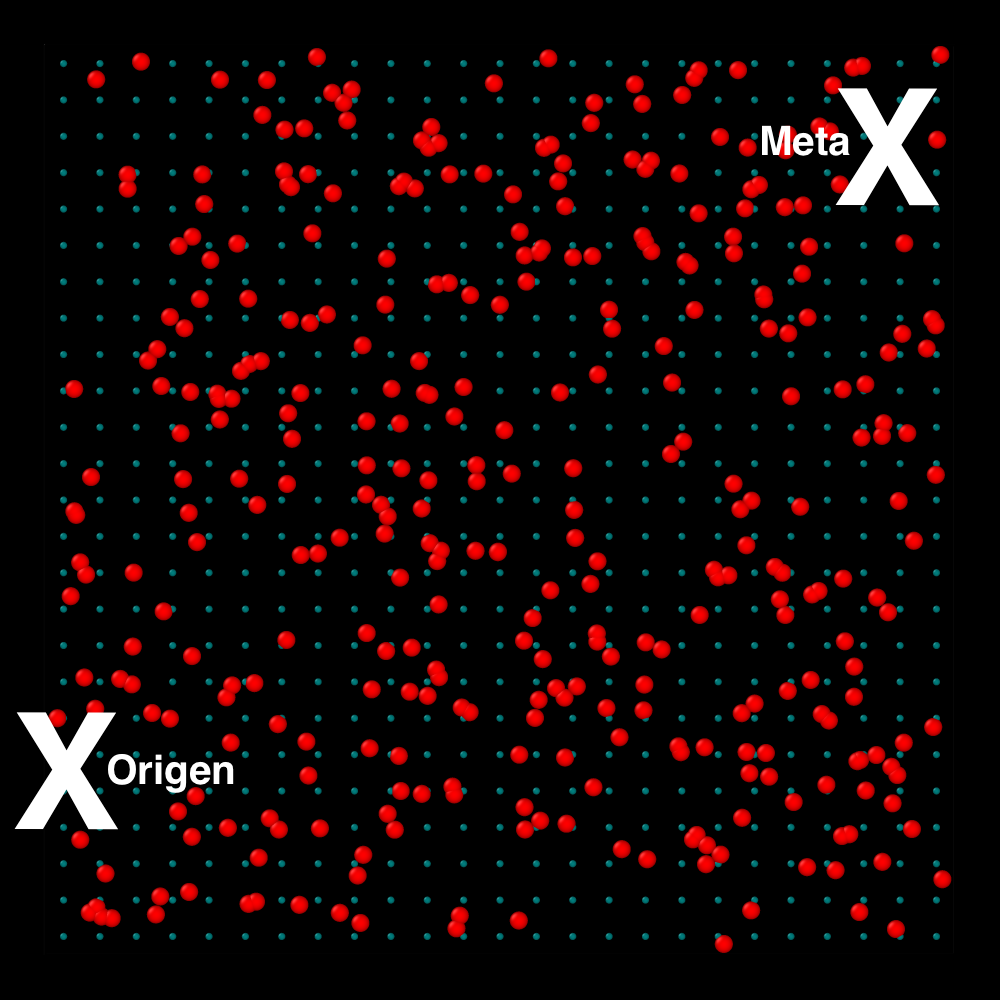
\includegraphics[width=0.75\textwidth]{images/scene.png}
\end{figure}
\end{frame}

\subsection{Heurística}

\begin{frame}
\frametitle{Métodos de Búsqueda Informado}
\framesubtitle{Introducción}
\begin{itemize}
	\item Sólo utilizando el costo $g(n)$, la búsqueda a ciegas resulta muy ineficiente
	\item Es necesario agregar valores que estimen cuánto falta para alcanzar el objetivo
	\item Definimos a una \textbf{heurística} $h(n) = $ costo estimado de la ruta más barata que une el estado del nodo $n$ con un estado meta
	\item Familia de algoritmos \textit{Best First}
\end{itemize}
\end{frame}

\begin{frame}
\frametitle{Métodos de Búsqueda Informado}
\framesubtitle{Mínimo Costo de Ruta}
	\begin{columns}[T]
		\begin{column}{.5\textwidth}
			$f(n) = g(n) + h(n)$
			
			\begin{itemize}
				\item $g(n):$ es el costo de la ruta que va del nodo inicial hasta $n$
				\item $h(n):$ estimación del mínimo costo de ruta que va de $n$ al nodo objetivo
				\item $f(n):$ costo estimado de la solución más barata que pasa por $n$
			\end{itemize}
			
			
		\end{column}
		\begin{column}{.5\textwidth}
    			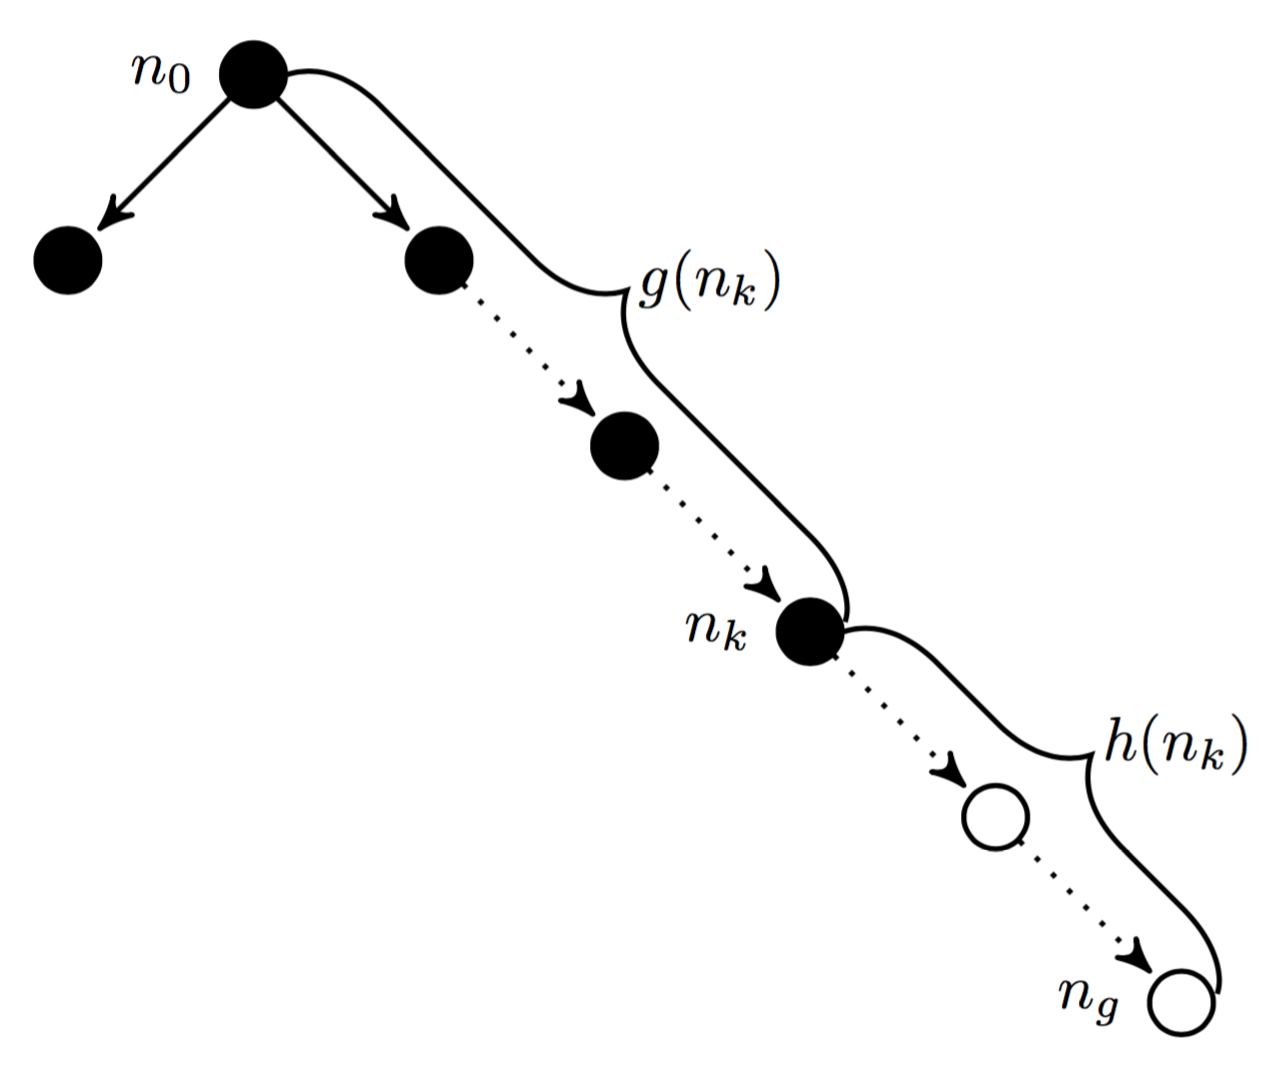
\includegraphics[width=\textwidth]{images/graph.png}
		\end{column}
	\end{columns}
\end{frame}

\begin{frame}
\frametitle{Método de Búsqueda Informado}
\framesubtitle{Algoritmo A*}
\begin{itemize}
	\item Actúa sobre un \textbf{grafo}
	\item El objetivo es encontrar el camino de \textbf{costo mínimo}
	\item Elige para expandir el nodo de menor $f$
\end{itemize}
\begin{block}{Adaptación necesaria}
Al actuar sobre un grafo el espacio de búsqueda debe ser \textbf{discreto}. Se requiere hacer una adaptación de la escena para poder discretizar posiciones de la habitación.
\end{block}
\end{frame}

\begin{frame}[plain]
\frametitle{Algoritmo A*}
\begin{enumerate}
\item Crear un árbol de búsqueda, $T_{r}$, que sólo esté formado por el nodo inicial $n_{0}$. Insertar $n{0}$ en la estructura FRONTERA.
\item Crear el conjunto EXPLORADOS, inicialmente vacío.
\item Si FRONTERA está vacía, el algoritmo termina con falla.
\item Extraer el primer nodo de FRONTERA e insertarlo en EXPLORADOS. Llamar a este nodo $n$.
\item Si $n$ es el nodo objetivo, salir del algoritmo y devolver la solución, que está formada por el camino definido por los arcos que llevan de $n$ a $n_{0}$ en el árbol $T_{r}$.
\item Expandir el nodo $n$ y generar el conjunto de nodos sucesores $M$. Incorporar los elementos de $M$ como sucesores de $n$ en el árbol $T{r}$, creando los arcos correspondientes entre $n$ y cada uno de los nodos de $M$.
\item \textbf{Reordenar FRONTERA de forma que primero estén los nodos de menor $f$}.
\item Ir al paso 3.
\end{enumerate}
\end{frame}

\begin{frame}
\frametitle{Algoritmo A*}
\framesubtitle{Comportamiento}
\begin{itemize}
	\item Una heurística es \textbf{admisible} si nunca sobreestima el costo real
	\item Si $h$ es admisible $\Rightarrow$ $f(n)$ nunca sobreestima el costo real de la mejor solución que pasa por $n$
	\item Con $h$ admisible A* es \textbf{completo} y \textbf{admisible}: Garantiza encontrar el camino óptimo al objetivo
\end{itemize}
\end{frame}

\begin{frame}
\frametitle{Adaptación}
\framesubtitle{Utilización de \textit{Waypoints}}
\begin{block}{Discretización de la escena}
\textit{Waypoints}: puntos $(x,y)$ por donde el agente podrá desplazarse. 

Estos serán los \textbf{nodos} por donde iterará el método de búsqueda.
\end{block}
\begin{itemize}
	\item Se decidió armar una \textbf{grilla} de \textit{waypoints} sobre la habitación
	\item Los \textit{waypoints} están separados unos de otros por una distancia $W_{d}$
\end{itemize}
\end{frame}

\begin{frame}
\frametitle{Adaptación}
\framesubtitle{Utilización de \textit{Waypoints}}
\begin{itemize}
	\item Cada \textit{waypoint} cuenta con una \textbf{ventana cuadrada de vecinos}
	\item $W_{v} :$ longitud del lado de la ventana
	\begin{itemize}
		\item $W_{v} = 3 :$ la ventana contiene a los 8 vecinos
		\item $W_{v} = 5 :$ la ventana contiene a los 24 vecinos
	\end{itemize}
	\item El conjunto de vecinos de la ventana del nodo $n$ constituye a los nodos sucesores del mismo
\end{itemize}
\end{frame}

\begin{frame}
\frametitle{Adaptación}
\framesubtitle{Utilización de \textit{Waypoints}}
\begin{itemize}
	\item Se utiliza $A*$ para obtener una lista de \textit{waypoints} por donde el agente tiene que transitar hasta alcanzar el nodo meta
	\item La lista de \textit{waypoints} obtenida se define como un conjunto de \textit{sub-objetivos} que tiene que ir alcanzando el agente
	\item Así, para cierto momento dado, el versor velocidad del agente tiene como dirección a la línea que se forma entre la posición actual del agente y el primer sub-objetivo
\end{itemize}
\end{frame}

\begin{frame}
\frametitle{Heurística}
\framesubtitle{Distancia al objetivo}
\begin{block}{Heurística propuesta}
$h(n)$ es la distancia real que se tiene al objetivo (distancia en línea recta al nodo meta)
\end{block}
\begin{itemize}
	\item $h(n)$ es admisible
	\item $g(n)$ es la distancia recorrida desde el nodo raíz hasta $n$
\end{itemize}
\end{frame}

\begin{frame}
\frametitle{Búsqueda limitada en profundidad}
\framesubtitle{Para el algoritmo $A*$}
\begin{itemize}
	\item El árbol de búsqueda tiene un \textbf{máximo de profundidad} $L$
	\item En el borde del límite se encuentra un nodo meta sub-óptimo
	\item Una vez alcanzado el sub-óptimo, \textbf{se reinicia la búsqueda} desde allí
\end{itemize}
\end{frame}

\begin{frame}
\frametitle{Detección de colisiones}
\framesubtitle{Poda del árbol de búsqueda del algoritmo $A*$}
\begin{itemize}
	\item Se genera un \textit{raycast} desde un waypoint origen hacia otro waypoint destino
	\item Si el trayecto del \textit{raycast} impacta sobre un obstáculo, entonces ese camino es \textbf{descartado} del árbol de búsqueda
	\item Así se evitan muchas colisiones innecesarias y caminos sin salida
\end{itemize}
\end{frame}

\begin{frame}
\frametitle{Prevención de colisiones}
\framesubtitle{Modificación del \textit{Contractile Particle Model}}
\begin{itemize}
	\item El objetivo es evitar los choques del agente con obstáculos que tiene en sus inmediaciones
	\item Con una partícula de radio $r_{p} = 1.1 r$ se calculan todos los posibles \textbf{solapamientos con obstáculos}
	\item Para cada solapamiento detectado se genera un versor director en dirección contraria a la del agente, para así evitar este obstáculo 
	\item Todos los versores se suman y se obtiene un \textbf{versor sumarizado} que representa la dirección a transitar para no colisionar con los obstáculos
\end{itemize}
\end{frame}

\subsection{Simulación}

\begin{frame}
\frametitle{Simulación}
\framesubtitle{Variables relevantes de la simulación}
\begin{itemize}
	\item $t$ $[s]$: Tiempo (en segundos) a visualizar.
	\item $dt$ $[s]$: Tiempo (en segundos) del paso de la simulación.
	\item $k$: Relación entre cantidad de pasos simulados y escritos para visualización.
\end{itemize}
\end{frame}

\begin{frame}[fragile]
\frametitle{Simulación}
\framesubtitle{Algoritmo de simulación}
\begin{lstlisting}[language=Java, caption = Algoritmo de simulación]
public void simulate(double t, double dt, int k){
	writeFrame(0);
	int framesWrited = 1;
	double totalTimeSimulated = 0;
	moveSystem(dt);
	totalTimeSimulated += dt;
	while(totalTimeSimulated < t){
		for(int i = 0; i < k; i++){
			moveSystem(dt);
			totalTimeSimulated += dt;
		}
		writeFrame(framesWrited++);
	}
}
\end{lstlisting}
\end{frame}

\begin{frame}
\frametitle{Simulación}
\framesubtitle{Parámetros de la simulación}
	\begin{itemize}
		\item $t < 100 s$ donde la simulación termina cuando el agente alcanza el nodo meta
		\item $3 < k < 7$
		\item $dt = 0.01 s$
	\end{itemize}
\end{frame}

\begin{frame}
\frametitle{Simulación}
\framesubtitle{Visualización}
\begin{itemize}
	\item La simulación y la visualización son independientes
	\item El algoritmo de simulación escribe un archivo \texttt{.tsv} con los siguientes datos:
	\begin{itemize}
		\item $(x,y)$
		\item $r$
		\item Color RGB para indicar las velocidades, donde R es la componente en el eje Y y G es la componente en eje X
	\end{itemize}
	\item Por último, se carga en \texttt{Ovito} el archivo de salida\texttt{.tsv} para realizar la visualización
\end{itemize}
\end{frame}

\section{Resultados}

\subsection{Gráficos y Tablas}

\begin{frame}
\Wider{
\frametitle{Gráfico de ?}
\framesubtitle{Para $? = ?$}
\begin{figure}[H]
	\centering
    \includegraphics[width=\textwidth]{example-image}
\end{figure}
}
\end{frame}

\begin{frame}
\frametitle{Tabla de ?}
\framesubtitle{Para distintos valores de ?}
\begin{center}
\begin{table}[h]
\centering
\adjustbox{max height=\dimexpr\textheight-3.0cm\relax,
           max width=\textwidth}{
\begin{tabular}{cc}
\hline
\textbf{?} & \textbf{?}\\ \hline
?&?\\ 
\end{tabular}
}
\caption{? para distintos valores de ?}
\end{table}
\end{center}
\end{frame}

\subsection{Animaciones}

\begin{frame}[plain]
\frametitle{Animación de la simulación}
\framesubtitle{Para $? = ?$}
\begin{figure}[H]
	\centering
%	\animategraphics[loop,controls,width=0.85\textwidth]{10}{animation/300n}{00001}{00242}
\end{figure}
\end{frame}

\subsection{Conclusiones}

\begin{frame}
\frametitle{Conclusiones}
\begin{itemize}
	\item Lorem
	\item Lorem
	\item Lorem
\end{itemize}	
\end{frame} 

\begin{frame}[plain]
    \centering
	\Huge Gracias
\end{frame}

\end{document}
